% Senseigigs — system workflow figure, research-paper style.
% Compile: pdflatex -interaction=nonstopmode senseigigs_workflow.tex
%
% WHY THIS IS NOT "A ROW OF BOXES": concrete data is drawn at every hop — the real
% gig text, real provider-id pills for each ranked list, a real feature vector for
% one example pair, real scored output rows — and every stage is a named container
% with its sub-modules visible.
%
% LAYOUT DISCIPLINE - the two things that made the earlier version ugly, both now fixed:
%   1. EVERY box style sets an explicit `text width`, so a box can never size itself
%      to its content and silently sprawl into the neighbouring band.
%   2. The input column, Stage 1, Stage 2 and Stages 3-4 each own a fixed x-band,
%      separated by >=16mm, and a container is fitted only around content already
%      inside its own band.
% verify with: python check_layout.py   (reports partial box overlaps + word collisions)
%
% Typesetting: hyphenation disabled inside nodes, explicit \\ breaks everywhere.
\documentclass[border=12pt]{standalone}
\usepackage[T1]{fontenc}
\usepackage{tikz}
\usetikzlibrary{arrows.meta, positioning, fit, backgrounds, calc, shapes.geometric}
\usepackage{amssymb}

\definecolor{ioC}{HTML}{2B6CB0}
\definecolor{retC}{HTML}{2F855A}
\definecolor{featC}{HTML}{B7791F}
\definecolor{rankC}{HTML}{C05621}
\definecolor{fuseC}{HTML}{6B46C1}
\definecolor{inkC}{HTML}{2D3748}
\definecolor{dataC}{HTML}{4A5568}
\definecolor{itemC}{HTML}{718096}
\definecolor{goodC}{HTML}{2F855A}

\begin{document}
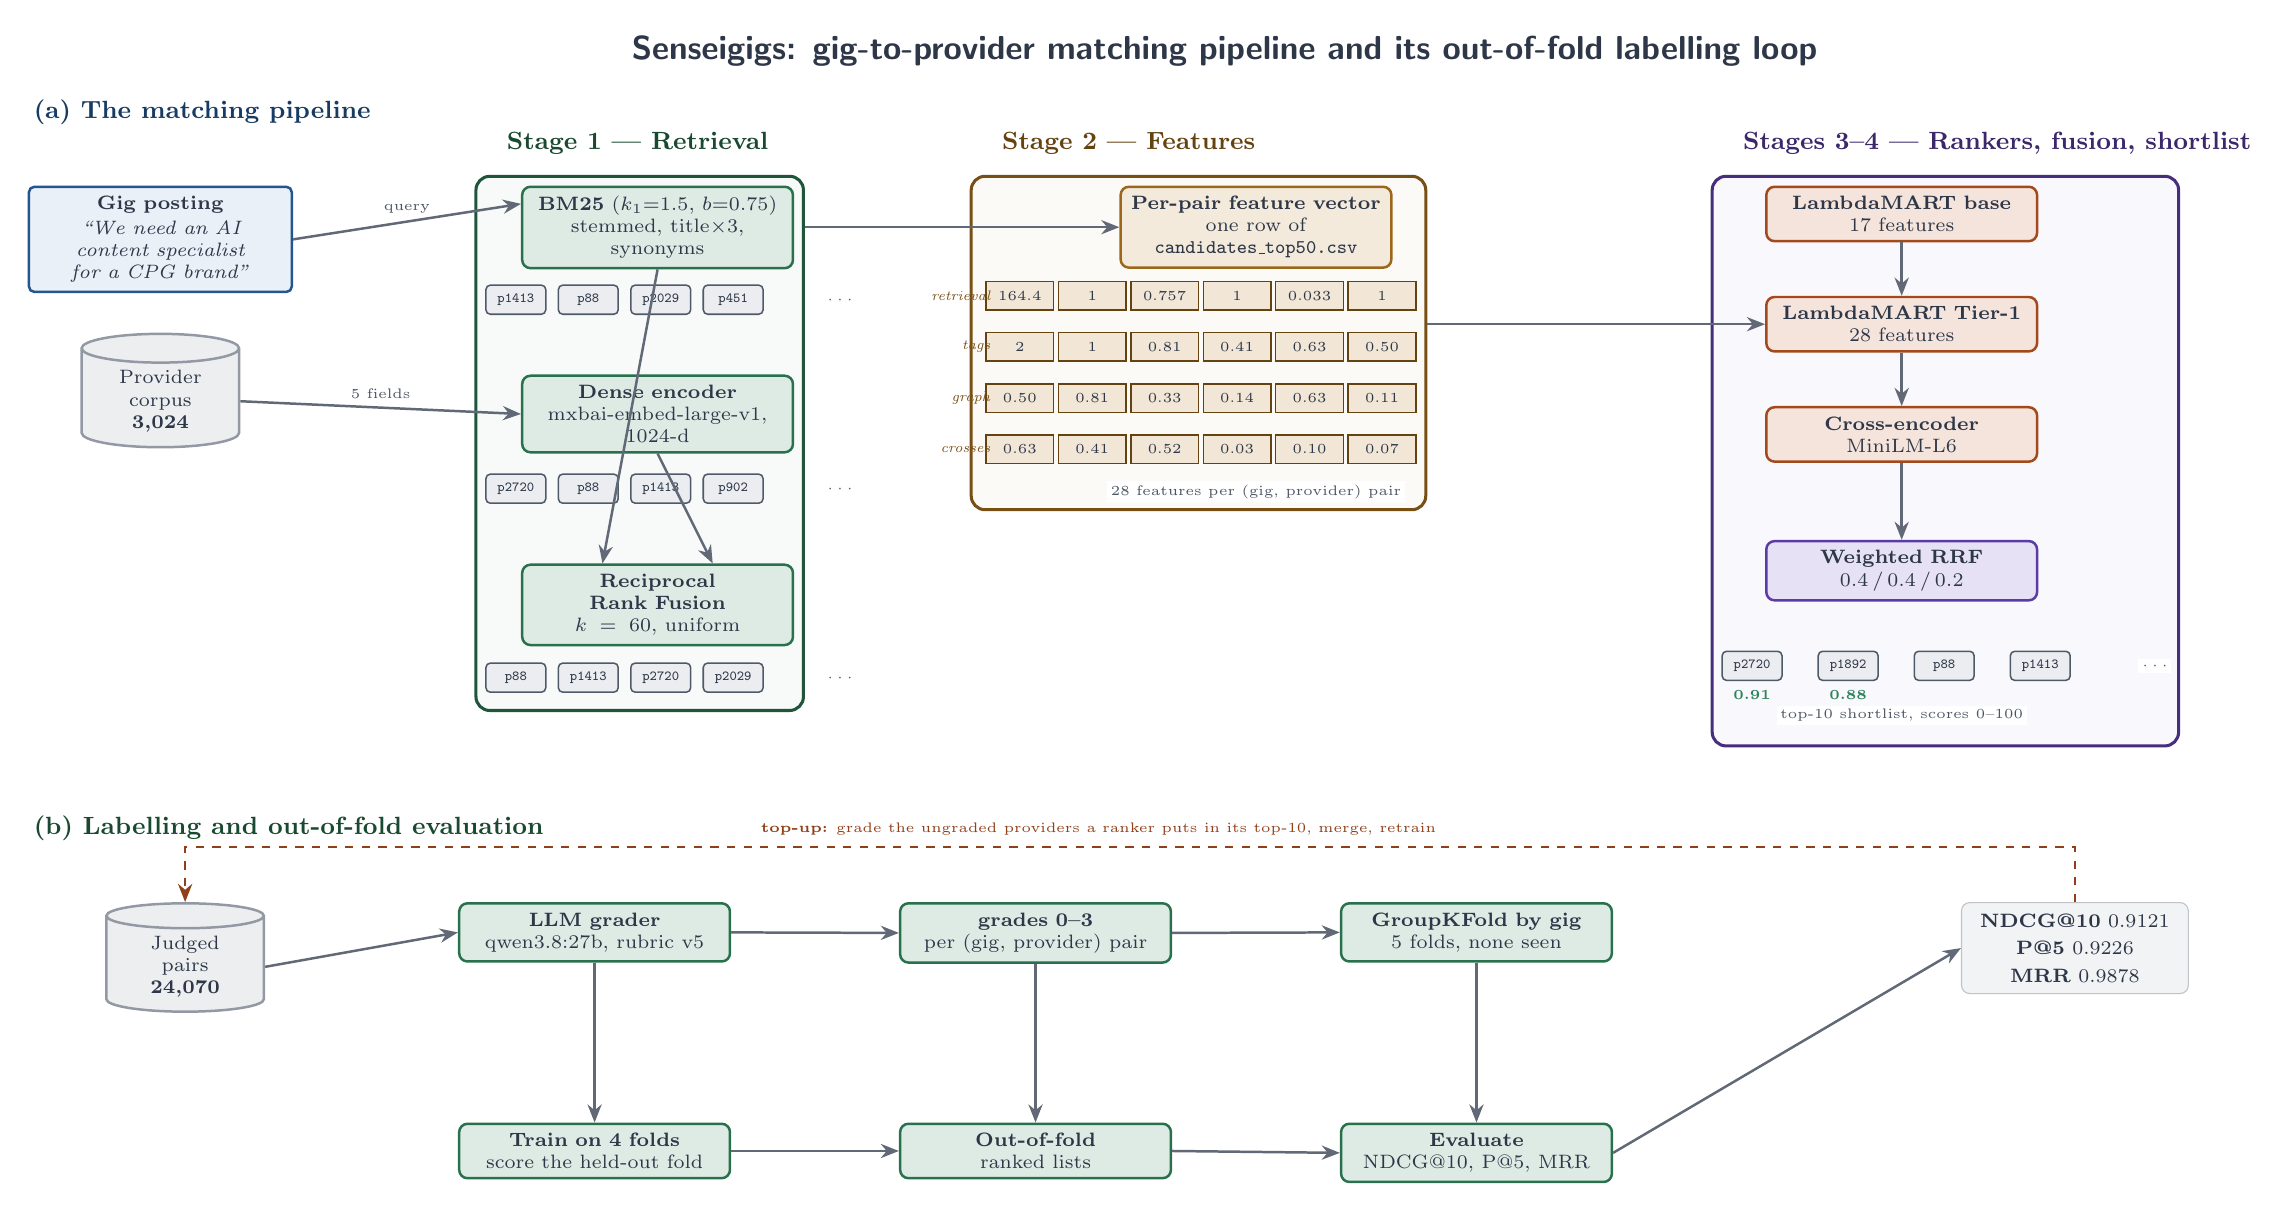
\begin{tikzpicture}[
  font=\sffamily,
  every node/.style={align=center,
    execute at begin node={\hyphenpenalty=10000\exhyphenpenalty=10000}},
  cont/.style={rounded corners=5pt, draw=#1!65!black, fill=#1!4, line width=1.1pt},
  ctitle/.style={font=\small\bfseries, text=#1!55!black},
  mod/.style={rounded corners=3pt, draw=#1!85!black, fill=#1!16, line width=0.9pt,
              inner sep=3.4pt, font=\scriptsize, text=inkC, text width=32mm},
  pill/.style={rounded corners=1.6pt, draw=itemC!70!black, fill=itemC!14, line width=0.55pt,
               inner sep=1.9pt, font=\tiny\ttfamily, text=inkC, minimum height=3.7mm,
               minimum width=7.6mm},
  card/.style={rounded corners=2pt, draw=ioC!80!black, fill=ioC!10, line width=0.9pt,
               inner sep=3.4pt, font=\scriptsize, text=inkC, text width=31mm},
  cyl/.style={cylinder, shape border rotate=90, aspect=0.30, draw=dataC!60, fill=dataC!10,
              line width=0.9pt, inner sep=2.4pt, font=\scriptsize, text=inkC,
              minimum height=12mm, minimum width=20mm},
  fcell/.style={draw=featC!55!black, fill=featC!18, line width=0.5pt, inner sep=1.4pt,
                font=\tiny, text=inkC, minimum height=3.6mm, minimum width=8.6mm},
  flab/.style={font=\tiny\itshape, text=featC!65!black},
  ar/.style={-{Stealth[length=2.3mm,width=1.8mm]}, line width=0.9pt, draw=inkC!75},
  arl/.style={font=\tiny, text=inkC!85, fill=white, inner sep=1.3pt},
  tb/.style={rounded corners=3pt, draw=inkC!30, fill=inkC!6, inner sep=4pt,
             font=\scriptsize, text=inkC, text width=26mm},
]

% ======================= TITLE =======================
\node[font=\sffamily\large\bfseries, text=inkC] at (0,6mm)
  {Senseigigs: gig-to-provider matching pipeline and its out-of-fold labelling loop};

% ============================================================
% PANEL (a) --- inference pipeline
% ============================================================
\node[ctitle=ioC, anchor=south west, inner sep=2pt] at (-152mm,-4mm)
  {(a) The matching pipeline};

% ---------- x-band A : inputs ----------
\node[card, anchor=north west] (gig) at (-152mm,-11mm)
  {\textbf{Gig posting}\\[1pt]
   \itshape ``We need an AI\\ content specialist\\ for a CPG brand''};
\node[cyl, anchor=north] (corpus) at ([yshift=-5mm]gig.south)
  {Provider\\corpus\\\textbf{3{,}024}};

% ---------- x-band B : Stage 1 (retrieval) ----------
\node[mod=retC, anchor=north] (bm25) at (-72mm,-11mm)
  {\textbf{BM25} ($k_1{=}1.5$, $b{=}0.75$)\\stemmed, title$\times$3, synonyms};
\foreach \t [count=\i] in {p1413,p88,p2029,p451} {%
  \pgfmathsetlengthmacro{\px}{-90mm + (\i-1)*9.2mm}%
  \node[pill] (b25-\i) at (\px,-25.5mm) {\t};}
\node[arl, anchor=west] at (-51mm,-25.5mm) {$\cdots$};

\node[mod=retC, anchor=north] (dense) at (-72mm,-35mm)
  {\textbf{Dense encoder}\\mxbai-embed-large-v1, 1024-d};
\foreach \t [count=\i] in {p2720,p88,p1413,p902} {%
  \pgfmathsetlengthmacro{\px}{-90mm + (\i-1)*9.2mm}%
  \node[pill] (dn-\i) at (\px,-49.5mm) {\t};}
\node[arl, anchor=west] at (-51mm,-49.5mm) {$\cdots$};

\node[mod=retC, anchor=north] (rrf1) at (-72mm,-59mm)
  {\textbf{Reciprocal Rank Fusion}\\$k=60$, uniform};
\foreach \t [count=\i] in {p88,p1413,p2720,p2029} {%
  \pgfmathsetlengthmacro{\px}{-90mm + (\i-1)*9.2mm}%
  \node[pill] (pool-\i) at (\px,-73.5mm) {\t};}
\node[arl, anchor=west] at (-51mm,-73.5mm) {$\cdots$};

\coordinate (s1bl) at (-93mm,-76.5mm);
\begin{pgfonlayer}{background}
  \node[cont=retC, fit=(bm25)(b25-1)(b25-4)(dense)(dn-1)(dn-4)(rrf1)(pool-1)(pool-4)(s1bl)] (S1) {};
\end{pgfonlayer}
\node[ctitle=retC, anchor=south west, inner sep=3pt] at ([xshift=3mm,yshift=1.5mm]S1.north west)
  {Stage 1 --- Retrieval};

% ---------- x-band C : Stage 2 (the per-pair feature vector) ----------
\node[mod=featC, anchor=north] (fx) at (4mm,-11mm)
  {\textbf{Per-pair feature vector}\\one row of \texttt{candidates\_top50.csv}};
\foreach \v [count=\i] in {164.4,1,0.757,1,0.033,1} {%
  \pgfmathsetlengthmacro{\px}{-26mm + (\i-1)*9.2mm}%
  \node[fcell] (fa-\i) at (\px,-25mm) {\v};}
\node[flab, anchor=east] at (-28.5mm,-25mm) {retrieval};
\foreach \v [count=\i] in {2,1,0.81,0.41,0.63,0.50} {%
  \pgfmathsetlengthmacro{\px}{-26mm + (\i-1)*9.2mm}%
  \node[fcell] (fb-\i) at (\px,-31.5mm) {\v};}
\node[flab, anchor=east] at (-28.5mm,-31.5mm) {tags};
\foreach \v [count=\i] in {0.50,0.81,0.33,0.14,0.63,0.11} {%
  \pgfmathsetlengthmacro{\px}{-26mm + (\i-1)*9.2mm}%
  \node[fcell] (fc-\i) at (\px,-38mm) {\v};}
\node[flab, anchor=east] at (-28.5mm,-38mm) {graph};
\foreach \v [count=\i] in {0.63,0.41,0.52,0.03,0.10,0.07} {%
  \pgfmathsetlengthmacro{\px}{-26mm + (\i-1)*9.2mm}%
  \node[fcell] (fd-\i) at (\px,-44.5mm) {\v};}
\node[flab, anchor=east] at (-28.5mm,-44.5mm) {crosses};
\node[arl, anchor=north] at (4mm,-48.5mm) {28 features per (gig, provider) pair};

\coordinate (s2bl) at (-31mm,-51mm);
\begin{pgfonlayer}{background}
  \node[cont=featC, fit=(fx)(fa-1)(fa-6)(fd-1)(fd-6)(s2bl)] (S2) {};
\end{pgfonlayer}
\node[ctitle=featC, anchor=south west, inner sep=3pt] at ([xshift=3mm,yshift=1.5mm]S2.north west)
  {Stage 2 --- Features};

% ---------- x-band D : Stages 3-4 ----------
\node[mod=rankC, anchor=north] (r1) at (86mm,-11mm) {\textbf{LambdaMART base}\\17 features};
\node[mod=rankC, anchor=north] (r2) at (86mm,-25mm) {\textbf{LambdaMART Tier-1}\\28 features};
\node[mod=rankC, anchor=north] (r3) at (86mm,-39mm) {\textbf{Cross-encoder}\\MiniLM-L6};
\node[mod=fuseC, anchor=north] (fus) at (86mm,-56mm) {\textbf{Weighted RRF}\\$0.4\,/\,0.4\,/\,0.2$};
\foreach \t [count=\i] in {p2720,p1892,p88,p1413} {%
  \pgfmathsetlengthmacro{\px}{67mm + (\i-1)*12.2mm}%
  \node[pill] (out-\i) at (\px,-72mm) {\t};}
\node[arl, anchor=west] at (116mm,-72mm) {$\cdots$};
\node[goodC, font=\tiny\bfseries, anchor=north] at (out-1.south) {0.91};
\node[goodC, font=\tiny\bfseries, anchor=north] at (out-2.south) {0.88};
\node[arl, anchor=north] at (86mm,-77mm) {top-10 shortlist, scores 0--100};
\coordinate (s4bl) at (64mm,-81mm);
\coordinate (s4r)  at (120mm,-68mm);
\begin{pgfonlayer}{background}
  \node[cont=fuseC, fit=(r1)(r2)(r3)(fus)(out-1)(out-4)(s4bl)(s4r)] (S4) {};
\end{pgfonlayer}
\node[ctitle=fuseC, anchor=south west, inner sep=3pt] at ([xshift=3mm,yshift=1.5mm]S4.north west)
  {Stages 3--4 --- Rankers, fusion, shortlist};

% ============================================================
% PANEL (b) --- labelling + out-of-fold loop
% ============================================================
\node[ctitle=goodC, anchor=south west, inner sep=2pt] at (-152mm,-95mm)
  {(b) Labelling and out-of-fold evaluation};

\node[cyl, anchor=north] (labels) at (-132mm,-102mm) {Judged\\pairs\\\textbf{24{,}070}};
\node[mod=goodC, anchor=north] (grader) at (-80mm,-102mm) {\textbf{LLM grader}\\qwen3.8:27b, rubric v5};
\node[mod=goodC, anchor=north] (grades) at (-24mm,-102mm) {\textbf{grades 0--3}\\per (gig, provider) pair};
\node[mod=goodC, anchor=north] (folds)  at (32mm,-102mm) {\textbf{GroupKFold by gig}\\5 folds, none seen};
\node[mod=goodC, anchor=north] (train)  at (-80mm,-130mm) {\textbf{Train on 4 folds}\\score the held-out fold};
\node[mod=goodC, anchor=north] (oof)    at (-24mm,-130mm) {\textbf{Out-of-fold}\\ranked lists};
\node[mod=goodC, anchor=north] (eval)   at (32mm,-130mm) {\textbf{Evaluate}\\NDCG@10, P@5, MRR};
\node[tb, anchor=north] (metrics) at (108mm,-102mm)
  {\textbf{NDCG@10} 0.9121\\[2pt]\textbf{P@5} 0.9226\\[2pt]\textbf{MRR} 0.9878};

% ---------- flows, panel (a) ----------
\draw[ar] (gig.east)    -- node[arl, midway, above, yshift=0.5mm] {query} ([yshift=3mm]bm25.west);
\draw[ar] (corpus.east) -- node[arl, midway, above, yshift=0.5mm] {5 fields} (dense.west);
\draw[ar] (bm25.south)  -- ([xshift=-7mm]rrf1.north);
\draw[ar] (dense.south) -- ([xshift=7mm]rrf1.north);
\draw[ar] (S1.east |- fx.west) -- (fx.west);
\draw[ar] (S2.east |- r2.west) -- (r2.west);
\draw[ar] (r1.south) -- (r2.north);
\draw[ar] (r2.south) -- (r3.north);
\draw[ar] (r3.south) -- (fus.north);

% ---------- flows, panel (b) ----------
\draw[ar] (labels.east)  -- (grader.west);
\draw[ar] (grader.east)  -- (grades.west);
\draw[ar] (grades.east)  -- (folds.west);
\draw[ar] (grader.south) -- (train.north);
\draw[ar] (grades.south) -- (oof.north);
\draw[ar] (folds.south)  -- (eval.north);
\draw[ar] (train.east)   -- (oof.west);
\draw[ar] (oof.east)     -- (eval.west);
\draw[ar] (eval.east)    -- (metrics.west);

% the top-up loop: this project's analogue of iterative self-improvement
\draw[ar, draw=rankC!75!black, dashed]
  (metrics.north) |- ([yshift=7mm]labels.north) -- (labels.north);
\node[arl, text=rankC!75!black, anchor=south] at (-16mm,-94mm)
  {\textbf{top-up:} grade the ungraded providers a ranker puts in its top-10, merge, retrain};

\end{tikzpicture}
\end{document}
